\documentclass[14pt]{article}
\usepackage{verbatim}
\usepackage{graphicx}
\usepackage{subcaption}
\usepackage{amsmath}

\title{CSE 300 Online 2}
\author{1605106}
\date{\today}

\begin{document}
	\maketitle
	\section{Graphics}
	Emacs, Nano, or Vim: Choose your Terminal-Based Text Editor Wisely. Nano
	is the built-in basic text editor for many popular distros. Its usually already
	contained in the distro, doesnt take any learning or getting used to, and all
	its commands and prompts are displayed at the bottom. Nano is the built-in
	basic text editor for many popular distros. Its usually already contained in the
	distro, doesnt take any learning or getting used to, and all its commands and
	prompts are displayed at the bottom. Vi or one of its variants typically comes
	with your distro-of-choice. Its considered a modal editor, which means there
	are different modes for navigating files and editing text. Because you navigate
	Vi most efficiently through the use of keyboard commands and shortcuts, Vi is
	better experienced than explained.
	\begin{figure}[h]
		\centering
		\begin{subfigure}{0.3\textwidth}
			
\includegraphics[width=0.8\textwidth]{emacslogo.png}
			\caption{Emacs}
		\end{subfigure}
		~
		\begin{subfigure}{0.3\textwidth}
			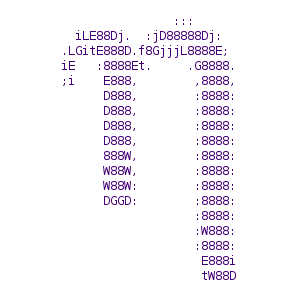
\includegraphics[width=0.8\textwidth]{nanologo.png}
			\caption{Nano}
		\end{subfigure}
		~
		\begin{subfigure}{0.3\textwidth}
			
\includegraphics[width=0.8\textwidth]{vimlogo.png}
			\caption{Vim}
		\end{subfigure}
	\caption{Terminal-based text-editors}
	\end{figure}

	\section{Equations}
	In algebra, a quadratic equation is any equation having the form $ax^2+bx+c=0$ where $x$ represents an unknown, and $a$, $b$, and $c$ represent known numbers, with
	$a\neq0$. It can easily be seen, by polynomial expansion, that the following
	equation is equivalent to the quadratic equation:
	$${\left(x+\frac{b}{2a}\right)}^2=\frac{b^2-4ac}{4a^2}$$
	
	Taking the square root of both sides, and isolating $x$, gives:
	\begin{equation}
		x = \frac{-b\pm\sqrt{b^2-4ac}}{2a}
	\end{equation}
	
	\section*{Some Equations:}
	$$f_1(t) = \int_{3}^{5}sin(x)dx$$
	
	$$F(x) = A_0 + \sum_{n=1}^{N}\left[A_ncos\left(\frac{2\pi nx}{P}\right)+B_nsin\left(\frac{2\pi nx}{P}\right)\right]$$
	
	$$\lim\limits_{x\rightarrow a}\frac{f(x)-f(a)}{x - a}$$
	
	$$\binom{a}{b + c} \binom{\frac{n^2-1}{2}}{n+1}$$
	
	$$h\leq \sqrt{\frac{(s-a)(s-b)(s-c)}{s}}$$
	
	$$6CO_2 + 6H_2O \rightarrow C_6H_{12}O_6 + 6O_2$$
	
	\begin{equation}
		\begin{bmatrix}
		a_1 & a_2 & a_3\\
		b_1 & b_2 & b_3\\
		c_1 & c_2 & c_3
		\end{bmatrix}
	\end{equation}
	
	
	
	
	
	
	
	
	\section{Bibliography}
	The recent success of neural networks has boosted research on pattern recog-
	nition and data mining. Many machine learning tasks such as object detection
	in “You Only Look Once” \cite{redmon2016you},machine translation \cite{luong2015effective}, and speech recognition \cite{hinton2012deep}, which once heavily relied on handcrafted feature engineering to extract in-
	formative feature sets, has recently been revolutionized by various end-to-end
	deep learning paradigms, i.e., convolutional neural networks (CNNs) \cite{lecun1995convolutional}, long
	shortterm memory (LSTM) \cite{hochreiter1997long}, and autoencoders.
	
	\bibliographystyle{plain}
	\bibliography{bibfile}
\end{document}